\documentclass{article}

\usepackage[UTF8]{ctex}
\usepackage{placeins}
\usepackage{graphicx}
\usepackage{listings}
\usepackage{xcolor} % 添加 xcolor 宏包
\lstset{ %
language=matlab,                % choose the language of the code
basicstyle=\footnotesize,       % the size of the fonts that are used for the code
numbers=left,                   % where to put the line-numbers
numberstyle=\footnotesize,      % the size of the fonts that are used for the line-numbers
stepnumber=1,                   % the step between two line-numbers. If it is 1 each line will be numbered
numbersep=5pt,                  % how far the line-numbers are from the code
backgroundcolor=\color{white},  % choose the background color. You must add \usepackage{color}
showspaces=false,               % show spaces adding particular underscores
showstringspaces=false,         % underline spaces within strings
showtabs=false,                 % show tabs within strings adding particular underscores
frame=single,           % adds a frame around the code
tabsize=2,          % sets default tabsize to 2 spaces
captionpos=b,           % sets the caption-position to bottom
breaklines=true,        % sets automatic line breaking
breakatwhitespace=false,    % sets if automatic breaks should only happen at whitespace
escapeinside={\%*}{*)}          % if you want to add a comment within your code
}
\title{hw08\_MATLAB}
\author{3220103167 缪晨轩}
\date{\zhdate{2024/5/18}}

\begin{document}
    \maketitle
    \section*{24}
        \begin{lstlisting}[caption={题24 MATLAB代码}, label={lst:matlab}]
            % 定义传递函数的分子和分母系数
            numerator = [1]; % 分子系数
            denominator = [1, 3, 3]; % 分母系数

            % 创建传递函数对象
            H = tf(numerator, denominator);

            % 绘制系统的冲激响应
            figure;
            impulse(H);
            title('系统的冲激响应');

            % 绘制系统的阶跃响应
            figure;
            step(H);
            title('系统的阶跃响应');

        \end{lstlisting}
        Answer: 
            \begin{figure}[h]
                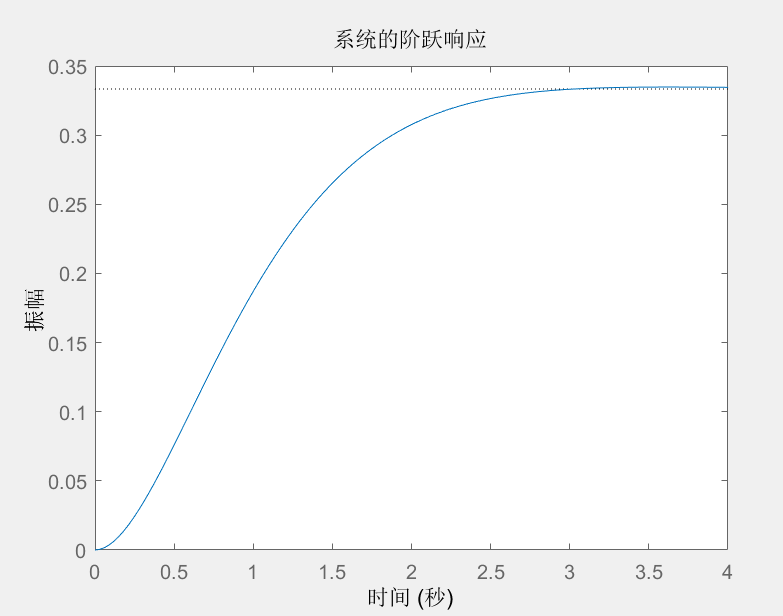
\includegraphics[scale=0.6]{24_1.png}
            \end{figure}
            \FloatBarrier
            \begin{figure}[h]
                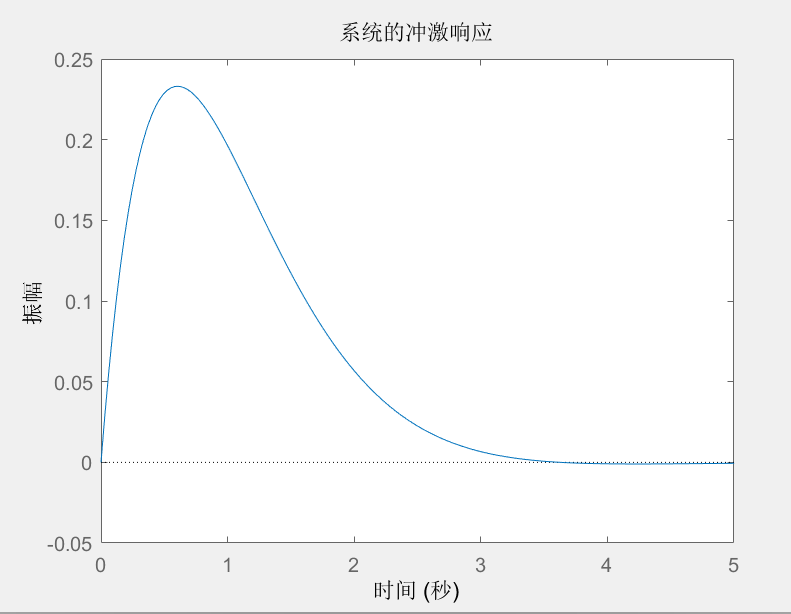
\includegraphics[scale=0.6]{24_2.png}
            \end{figure}
            \FloatBarrier
    \section*{27}
        \begin{lstlisting}[caption={题27 MATLAB代码}, label={lst:matlab}]
            % 参数定义
            omega_0 = 1; % 可以根据需要调整omega_0的值
            t = -10:0.01:10; % 定义时间轴,时间范围和步长可以根据需要调整

            % 定义单位冲激响应 h(t)
            h_t = 1 ./ (pi * t);
            h_t(t == 0) = 0; % 处理 t = 0 处的值

            % 定义输入信号 x(t)
            x_t = cos(omega_0 * t);

            % 计算卷积 y(t)
            y_t = conv(x_t, h_t, 'same') * (t(2) - t(1)); % 卷积结果和时间步长相乘

            % 绘图
            figure;
            plot(t, y_t);
            title('滤波器的零状态响应 y(t)');
            xlabel('时间 t');
            ylabel('响应 y(t)');
            grid on;


        \end{lstlisting}
        Answer:
            \begin{figure}[h]
                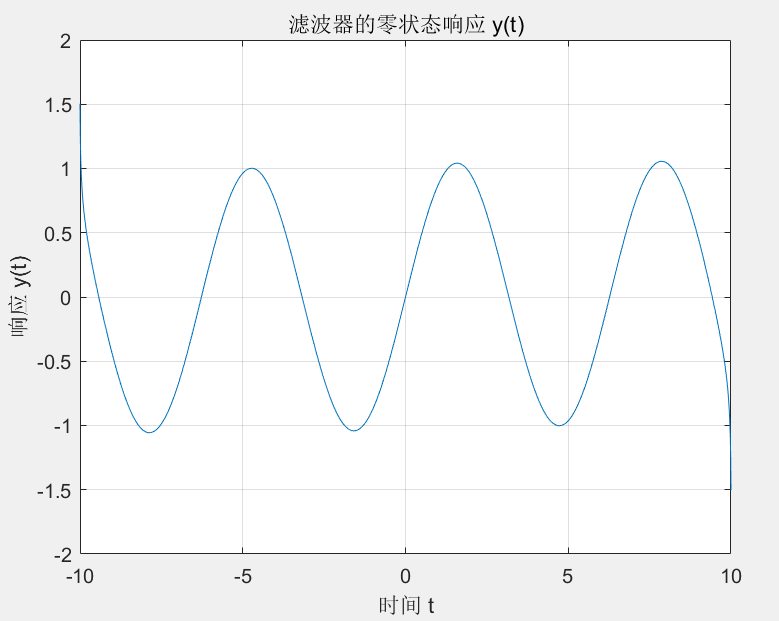
\includegraphics[scale=0.6]{27.png}
            \end{figure}
            \FloatBarrier
            
    
\end{document}